\section{Walter, Carrier - Rapid acceleration in dogs: ground reaction forces and posture dynamics - 2009}

\subsection*{Summary}

\begin{multicols}{2}
[
Steady-state locomotion compared to rapid accelerations:
]
\textbf{Steady-state locomotion:}
\begin{itemize}
\item Front legs support 56-64 \% of the body weight
\item On humans it was observed that also legs stiffness is correlated to maximum speed, besides power and strenght. For rapid accelerations instead stiffness plays no role.
\item Duty factors are much lower (shorter stance phase) even for ''long-stance'' gaits such as trot and pace
\end{itemize}
\columnbreak

\textbf{Rapid accelerations:}
\begin{itemize}
\item Front legs support 43 \% of the body weight
\item Limbs are more retracted and flexed in order to use all the range of motion. The propulsive force is thus produced for a larger range of motion.
\item Trunk experiences greater pitching movement
\item Much higher force peaks (2 or 3 times higher)
\item Ground forces are entirely propulsive (almost no braking in the first steps).
\item Half-bound was the preferred gait
\item vertical forces in fore limbs increase step by step together with speed and stance time decreases.
\item angular excursion of about $28\degree$ which is 38 \% more than the excursion of steady-state
\item the \textit{head-end down} configuration (positive pitch) helps to lower down the CoM and thus bring the GRF alligned to the CoM.
\item The optimal swing time is simply the shortest time required to reposition the legs (internal work). \textbf{The shorter is the swing time, the better.}
\end{itemize}

\end{multicols}

\begin{figure}[h]
  \centering
  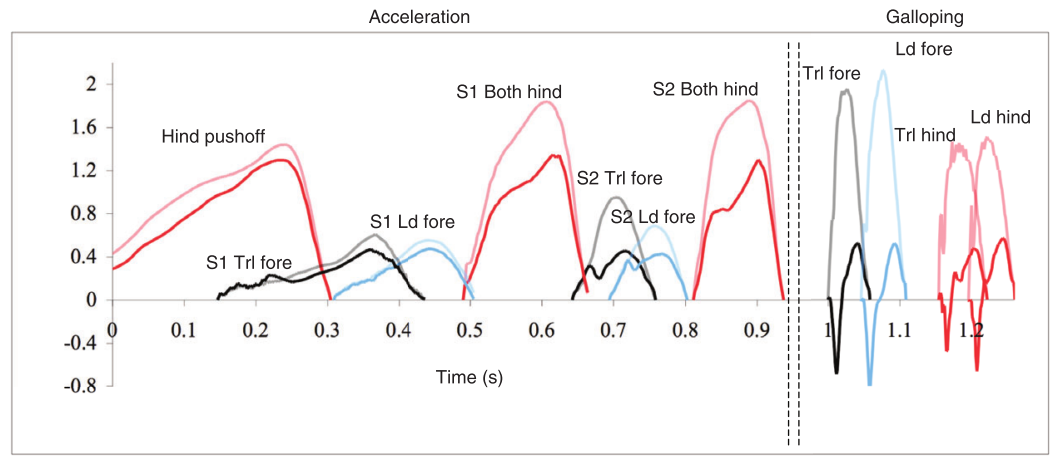
\includegraphics[width=150mm]{figs/RapidAccelerations}
  \caption{Rapid accelerations on dogs: this plots refer to a \textbf{half-bounding gait (hind legs move together while front legs are sequential: leading+trailing leg)}}
  \label{RapAcc}
\end{figure}
\subsection*{Experimental observations}
\begin{multicols}{3}
\textbf{Front legs:}
\begin{enumerate}
\item No braking forces were applied with the forelimbs during the first two accelerating strides.
\item stance time decreases when speed increases
\item vertical ground force of fore limbs increases with speed.
\end{enumerate}
\columnbreak

\textbf{Hind legs:}
\begin{enumerate}
\item The highest vertical ground forces are measured in the second step, as they decrease when the gait goes to steady state.
\item stance time decreases when speed increases
\item The orientation of the hind ground forces is strikingly constant
\item greater force is produced in the last part of the stance when joints are extending more rapidly
\end{enumerate}
\columnbreak

\textbf{Pitch:}
\begin{enumerate}
\item To avoid net pitching of the torso during locomotion, a quadruped’s net ground reaction force vector must pass through its center of mass.
\item The unavoidable pitching motion at start is slowly converted into linear speed when the dog reaches the steady state speed.
\end{enumerate}



\end{multicols}
